% ---------------------------------------------------------------------------------------------------------------
% TEMPLATE PARA TRABALHO DE CONCLUSÃO DE CURSO
% Universidade Tecnológica Federal do Paraná - UTFPR
% Customização da classe abnTeX2 (http://www.abntex.net.br/) para as normas da UTFPR
%
% ADAPTADO DO Projeto hospedado em: <link git>
% Autores: Diego Marczal  <>
% 	   Michael Vornes <https://github.com/mvornes>
%
%----------------------------------------------------------------------------------------------------------------
% Codificação: UTF-8
% LaTeX:  abnTeX2          
% ---------------------------------------------------------------------------------------------------------------
\title{templateBSI}


% CARREGA CLASSE PERSONALIZADA DA UTFPR--------------------------------------------------------------------------
\documentclass[%twoside,                   % Impressão em frente e verso
    	        oneside,                   % Impressão apenas frente
]{configuracoes/utfpr-abntex2}


% INCLUI ARQUIVOS DE CONFIGURAÇÕES-------------------------------------------------------------------------------
% REFERÊNCIAS------------------------------------------------------------------
\usepackage[%
    alf,
    abnt-emphasize=bf,
    bibjustif,
    recuo=0cm,
    abnt-url-package=url,       % Utiliza o pacote url
    abnt-refinfo=yes,           % Utiliza o estilo bibliográfico abnt-refinfo
    abnt-etal-cite=3,
    abnt-etal-list=3,
    abnt-thesis-year=final
]{abntex2cite}                  % Configura as citações bibliográficas conforme a norma ABNT

% PACOTES----------------------------------------------------------------------
\usepackage[final]{pdfpages}
\usepackage{booktabs}                                       % Réguas horizontais em tabelas
\usepackage{color, colortbl}                                % Controle das cores
\usepackage{float}                                          % Necessário para tabelas/figuras em ambiente multi-colunas
\usepackage{graphicx}                                       % Inclusão de gráficos e figuras
\usepackage{icomma}                                         % Uso de vírgulas em expressões matemáticas
\usepackage{indentfirst}                                    % Indenta o primeiro parágrafo de cada seção
\usepackage{microtype}                                      % Melhora a justificação do documento
\usepackage{multirow, array}                                % Permite tabelas com múltiplas linhas e colunas
\usepackage{subeqnarray}                                    % Permite subnumeração de equações
\usepackage{lastpage}                                       % Para encontrar última página do documento
\usepackage{verbatim}                                       % Permite apresentar texto tal como escrito no documento, ainda que sejam comandos Latex
\usepackage{amsfonts, amssymb, amsmath}                     % Fontes e símbolos matemáticos
\usepackage[algoruled, portuguese]{algorithm2e}             % Permite escrever algoritmos em português
\usepackage[scaled]{helvet}                                % Usa a fonte Helvetica
%\usepackage{times}                                          % Usa a fonte Times
%\usepackage{palatino}                                      % Usa a fonte Palatino
%\usepackage{lmodern}                                       % Usa a fonte Latin Modern
\usepackage[bottom]{footmisc}                               % Mantém as notas de rodapé sempre na mesma posição
\usepackage{ae, aecompl}                                    % Fontes de alta qualidade
\usepackage{latexsym}                                       % Símbolos matemáticos
\usepackage{lscape}                                         % Permite páginas em modo "paisagem"
%\usepackage{picinpar}                                      % Dispor imagens em parágrafos
%\usepackage{scalefnt}                                      % Permite redimensionar tamanho da fonte
\usepackage{subfig}                                        % Posicionamento de figuras
%\usepackage{upgreek}                                       % Fonte letras gregas
%pra codigo python
\usepackage{listings}
\usepackage{pdfpages}
\usepackage{lipsum}
\usepackage[utf8]{inputenc}
\usepackage[brazil]{babel}
\usepackage[T1]{fontenc}
\usepackage{lmodern}
\usepackage{easylist} %para aninhar enumerate
\usepackage{paralist} %para compactenum



\lstset{language=C,
keywords={do, break,case,catch,continue,else,elseif,end,for,function,global,if,otherwise,persistent,return,switch,try,while,int, float, char},
basicstyle = \ttfamily, % \footnotesize, % Tamanho da fonte do código
numbers = left, % Posição da numeração das linhas
numberstyle = \tiny\color{blue}, % Estilo da numeração de linhas
stepnumber = 1, % Numeração das linhas ocorre a cada quantas linhas?
numbersep = 10pt, % Distância entre a numeração das linhas e o código
backgroundcolor = \color{white}, % Cor de fundo
showspaces = false, % Exibe espaços com um sublinhado
showstringspaces = false, % Sublinha espaços em Strings
showtabs = false, % Exibe tabulação com um sublinhado
%frame = single, % Envolve o código com uma moldura, pode ser single ou trBL
%rulecolor = \color{black}, % Cor da moldura
tabsize = 2, % Configura tabulação em x espaços
captionpos = b, % Posição do título pode ser t (top) ou b (bottom)
breaklines = true, % Configura quebra de linha automática
breakatwhitespace= false, % Configura quebra de linha
title = \lstname, % Exibe o nome do arquivo incluido
%caption = \lstname, % Também é possível usar caption no lugar de title
keywordstyle = \color{blue}, % Estilo das palavras chaves
commentstyle = \color{gray}, % Estilo dos Comentários
}

% Seleção de código de fonte
% Redefine a fonte para uma fonte similar a Arial (fonte Helvetica)
%\renewcommand*\familydefault{\sfdefault}

% CONFIGURAÇÕES DE APARÊNCIA DO PDF FINAL--------------------------------------
\makeatletter
\hypersetup{%
    portuguese,
    colorlinks=true,   % true: "links" coloridos; false: "links" em caixas de texto
    linkcolor=black,    % Define cor dos "links" internos
    citecolor=black,    % Define cor dos "links" para as referências bibliográficas
    filecolor=black,    % Define cor dos "links" para arquivos
    urlcolor=black,     % Define a cor dos "hiperlinks"
    breaklinks=true,
    pdftitle={\@title},
    pdfauthor={\@author},
    pdfkeywords={abnt, latex, abntex, abntex2}
}
\makeatother

% ALTERA O ASPECTO DA COR AZUL--------------------------------------------------
\definecolor{blue}{RGB}{41,5,195}

% REDEFINIÇÃO DE LABELS---------------------------------------------------------
\renewcommand{\algorithmautorefname}{Algoritmo}
\def\equationautorefname~#1\null{Equa\c c\~ao~(#1)\null}

\captionsetup{position=bottom}

% CRIA ÍNDICE REMISSIVO---------------------------------------------------------
\makeindex

% HIFENIZAÇÃO DE PALAVRAS QUE NÃO ESTÃO NO DICIONÁRIO---------------------------
\hyphenation{%
    qua-dros-cha-ve
    Kat-sa-gge-los
}



% INCLUI ARQUIVOS DO TRABALHO DE CONCLUSÃO DE CURSO (PRÉ-TEXTUAIS, TEXTUAIS, PÓS-TEXTUAIS)-----------------------

% INSERE CAPA E FOLHA DE ROSTO
% CAPA---------------------------------------------------------------------------------------------------

% ORIENTAÇÕES GERAIS-------------------------------------------------------------------------------------
% Caso algum dos campos não se aplique ao seu trabalho, como por exemplo,
% se não houve coorientador, apenas deixe vazio.
% Exemplos: 
% \coorientador{}
% \departamento{}

% DADOS DO TRABALHO--------------------------------------------------------------------------------------
\titulo{Análise do desempenho de protocolos para computação em névoa com o uso de dispositivos móveis}
%Termografia Dinâmica para Auxílio na detecção de indicadores de Câncer de Mama
\titleabstract{Título em inglês}
\autor{José Vitor Moreno\\Luís Henrique Beltrão Santana}
\autorcitacao{Moreno,José; Santana, Luís} % Sobrenome em maiúsculo
\local{Curitiba}
\data{2021}

% NATUREZA DO TRABALHO-----------------------------------------------------------------------------------
% Opções: 
% - Trabalho de Conclusão de Curso (se for Graduação)
% - Dissertação (se for Mestrado)
% - Tese (se for Doutorado)
% - Projeto de Qualificação (se for Mestrado ou Doutorado)
\projeto{Trabalho de Conclusão de Curso}

% TÍTULO ACADÊMICO---------------------------------------------------------------------------------------
% Opções:
% - Bacharel ou Tecnólogo (Se a natureza for Trabalho de Conclusão de Curso)
% - Mestre (Se a natureza for Dissertação)
% - Doutor (Se a natureza for Tese)
% - Mestre ou Doutor (Se a natureza for Projeto de Qualificação)
\tituloAcademico{Bacharel}

% ÁREA DE CONCENTRAÇÃO E LINHA DE PESQUISA---------------------------------------------------------------
% Se a natureza for Trabalho de Conclusão de Curso, deixe ambos os campos vazios
% Se for programa de Pós-graduação, indique a área de concentração e a linha de pesquisa
\areaconcentracao{}
\linhapesquisa{}

% DADOS DA INSTITUIÇÃO-----------------------------------------------------------------------------------
% Se a natureza for Trabalho de Conclusão de Curso, coloque o nome do curso de graduação em "programa"
% Formato para o logo da Instituição: \logoinstituicao{<escala>}{<caminho/nome do arquivo>}
\instituicao{Universidade Tecnológica Federal do Paraná}
\departamento{DAINF - Departamento Acadêmico de Informática}
\programa{Curso de Engenharia de Computação}
\logoinstituicao{0.2}{dados/figuras/logo-instituicao.png} 

% DADOS DOS ORIENTADORES---------------------------------------------------------------------------------
%\orientador[Orientador:]{Nome do orientador}
\orientador[Orientadora:]{profª. Drª. Ana Cristina Kochem Vendramin}
\instOrientador{DAINF - Departamento Acadêmico de Informática -UTFPR}

\coorientador{prof. PhD. Daniel Fernando Pigatto}
%\coorientador[Coorientadora:]{Nome da coorientadora}
\instCoorientador{DAINF - Departamento Acadêmico de Informática -UTFPR}

% FOLHA DE ROSTO--------------------------------------------------------------------------------------------------------

% TRABALHO DE CONCLUSÃO DE CURSO
\preambulo{Proposta de {\imprimirprojeto} apresentado ao {\imprimirprograma} da {\imprimirinstituicao}, como requisito parcial para a obtenção do título de {\imprimirtituloAcademico}.}

% DISSERTAÇÃO DE MESTRADO
% \preambulo{{\imprimirprojeto} apresentada ao Programa de \mbox{Pós-graduação} da {\imprimirinstituicao}, como requisito parcial para obtenção do título de {\imprimirtituloAcademico}.}

% TESE DE DOUTORADO
% \preambulo{{\imprimirprojeto} apresentada ao Programa de \mbox{Pós-graduação} da {\imprimirinstituicao}, como requisito parcial para a obtenção do título de {\imprimirtituloAcademico}.}

% PROJETO DE QUALIFICAÇÃO DE MESTRADO OU DOUTORADO
%\preambulo{{\imprimirprojeto} apresentado ao Programa de \mbox{Pós-graduação} da {\imprimirinstituicao}, como requisito parcial para a obtenção do título de {\imprimirtituloAcademico}.}

% OBSERVAÇÕES-----------------------------------------------------------------------------------------------------------
% Altere este arquivo APENAS comentando as linhas que não se aplicam ao tipo de trabalho acadêmico desejado.



\usepackage[T1]{fontenc}
\begin{document}

\pretextual
\imprimircapa                                               	           % Comando para imprimir Capa
% * <brunops96@gmail.com> 2018-03-20T21:12:11.668Z:
%
% ^.
\imprimirfolhaderosto{}                                     		   % Comando para imprimir Folha de rosto
% INSERE ELEMENTOS PRÉ-TEXTUAIS
%% DEDICATÓRIA------------------------------------------------------------------

\renewcommand{\dedicatorianame}{DEDICATÓRIA}

\begin{dedicatoria}

Altere este texto inserindo a dedicatória do seu trabalho. 

\end{dedicatoria}
          			   % Dedicatória
%% AGRADECIMENTOS---------------------------------------------------------------

\begin{agradecimentos}[AGRADECIMENTOS]

Edite e coloque aqui os agradecimentos às pessoas e/ou instituições que contribuíram para a realização do trabalho.

É obrigatório o agradecimento às instituições de fomento à pesquisa que financiaram total ou parcialmente o trabalho, inclusive no que diz respeito à concessão de bolsas.

\end{agradecimentos}
        			   % Agradecimentos
%% EPÍGRAFE---------------------------------------------------------------------

\renewcommand{\epigraphname}{EPÍGRAFE}

\begin{epigrafe}

\textit{Altere o texto para inserir a epígrafe do seu trabalho.}

\end{epigrafe}

% OBSERVAÇÕES------------------------------------------------------------------
% Altere o texto para inserir a epígrafe do seu trabalho

              			   % Epígrafe
%
%% -----------------------------------------------------------------------------
% Folha de Aprovação
% -----------------------------------------------------------------------------

\textopadraofolhadeaprovacao{Esta folha deverá ser substituída pela cópia digitalizada da folha de aprovação fornecida.}
\clearpage
\newpage\ \newpage
% -----------------------------------------------------------------------------
% Este documento foi mantido apenas para preservar a paginação do trabalho
% acadêmico final, após a inserção da folha de aprovação fornecida
% -----------------------------------------------------------------------------
 

%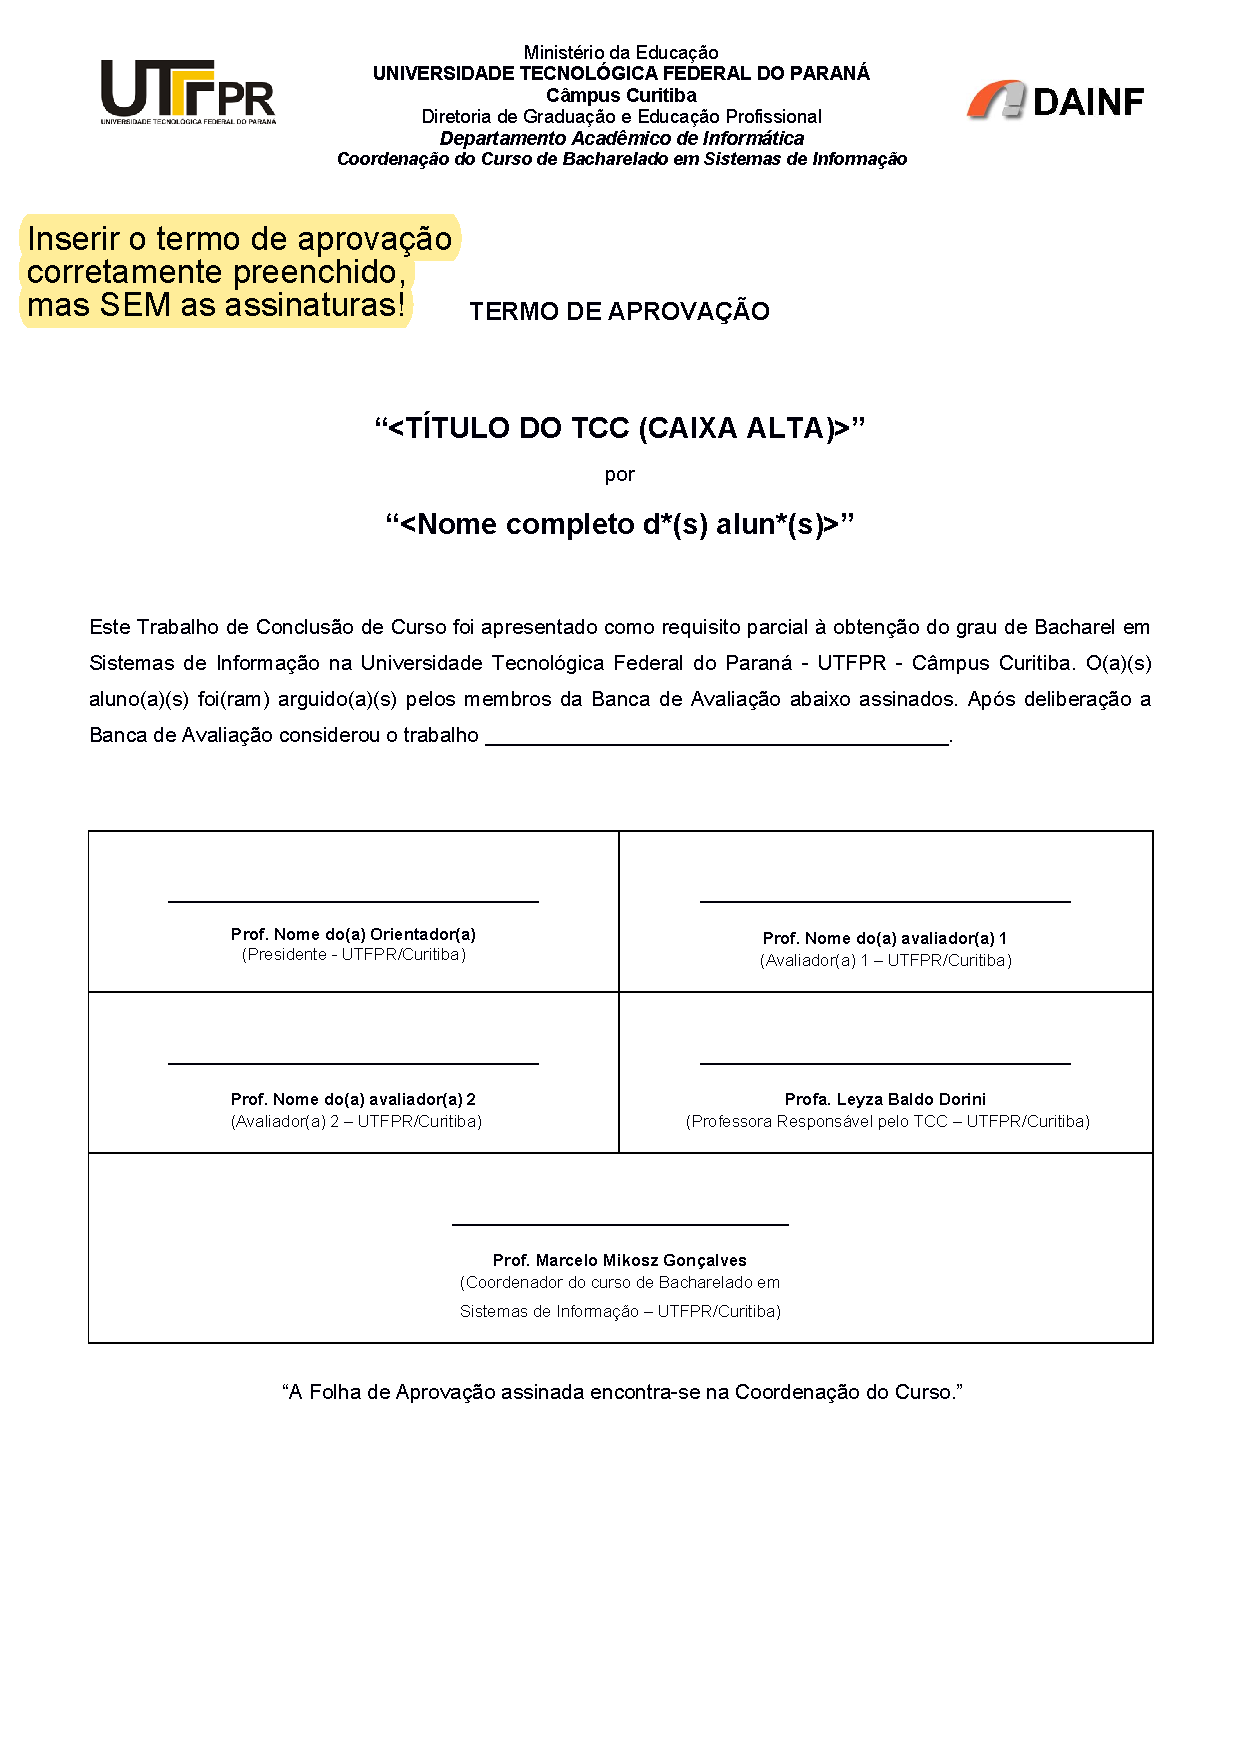
\includepdf[pages=-,pagecommand={},width=\textwidth]{dados/FOLHA_APROVACAO.pdf}

% RESUMO--------------------------------------------------------------------------------

\begin{resumo}[RESUMO]
\begin{SingleSpacing}

% Não altere esta seção do texto--------------------------------------------------------
\imprimirautorcitacao. \imprimirtitulo. \imprimirdata. \pageref {LastPage} f. \imprimirprojeto\ – \imprimirprograma, \imprimirinstituicao. \imprimirlocal, \imprimirdata.\\
%---------------------------------------------------------------------------------------

Com o avanço do poder de processamento e a miniaturização dos processadores modernos, a cada ano que se passa, vê-se cada vez mais dispositivos portáteis se tornando populares no Brasil. Esses dispositivos se utilizam de sistemas embarcados onde o consumo de recursos como bateria, processamento e memória, que são escassos, são de vital importância para que o usuário tenha uma boa experiência de uso. Atualmente, os dispositivos móveis são uma grande fonte de geração de dados. Esses dados ficam situados nas bordas da rede, sendo muitas vezes inviável tentar centralizá-los. A camada de computação em névoa surgiu como um meio de prover serviços de armazenamento e comunicação entre a computação em nuvem e os dispositivos finais (IoT - Internet of Things), podendo fornecer dados em tempo real de forma descentralizada e escalável.  Um elemento chamado servidor de mensagens fica responsável por gerenciar e distribuir a informação através de um ou mais canais de comunicação, de modo a demandar menos recursos computacionais com requisições repetidas para uma mesma informação. Este trabalho visa analisar alguns protocolos de comunicação para computação em névoa, como MQTT (Message Queuing Telemetry Transport), AMQP (Advanced Message Queuing Protocol) e STOMP (Simple Text Orientated Messaging Protocol) por meio de um servidor de mensagens RabbitMQ. O objetivo é analisar como esses protocolos se comportam nesse novo mundo desafiador de recursos escassos, que são autogerenciados por ferramentas internas do Sistema Operacional.  

\textbf{Palavras-chave}: Computação em névoa, Dispositivos Móveis, AMQP, STOMP, MQTT. 
% Escolha de 3 a 5 palavras ou termos que descrevam bem o seu trabalho 
\end{SingleSpacing}
\end{resumo}


             			   % Resumo em Português
%
% ABSTRACT--------------------------------------------------------------------------------

\begin{resumo}[ABSTRACT]
\begin{SingleSpacing}

% Não altere esta seção do texto--------------------------------------------------------
\imprimirautorcitacao. \imprimirtitleabstract. \imprimirdata. \pageref {LastPage} f. \imprimirprojeto\ – \imprimirprograma, \imprimirinstituicao. \imprimirlocal, \imprimirdata.\\
%---------------------------------------------------------------------------------------

With the advancement of processing capacity and the miniaturization of modern processors, with each passing year it's noticeable how much popular the mobile devices are becoming in Brazil. This devices uses embedded systems, where the consumption of resources like batery, processement power and memory, which are scarce, have a vital importance in order to provide a good experience to the user. Currently, mobile devices are a great source of data generation. This data are usually located at the edges of the network, and it is often unfeasible to try to centralize. The fog computing layer was created as a means of providing storage and communication services between cloud computing and the end devices (IoT - Internet of Things), being able to provide real-time data in a decentralized and scalable way. An element called message broker is responsible for managing and distributing information through one or more communication channels, in order to demand less computational resources with repeated requests for a single information. This paper will aim to analyze some communication protocols for fog computing, such as MQTT (Message QueuingTelemetry Transport), AMQP (Advanced Message Queuing Protocol) e STOMP (SimpleText Orientated Messaging Protocol) through the Broker RabbitMQ, in order to analyze how these protocols behave in this challenging new world of scarce resources, which are self-managed by Internal tools of the Operating System.\par

\textbf{Keywords}: Fog computing. Android. Smartphone, AMQP, STOMP, MQTT. 
% Escolha de 3 a 5 palavras ou termos que descrevam bem o seu trabalho 

\end{SingleSpacing}
\end{resumo}


             		           % Resumo em Inglês
% Lista de Figuras----------------------------------------------------------------

\pdfbookmark[0]{\listfigurename}{lof}
\listoffigures*
\cleardoublepage

% OBSERVAÇÕES---------------------------------------------------------------------
% Este arquivo não precisa de ser alterado, pois a lista é gerada automaticamente.
   % Lista de Figuras
% LISTA DE QUADROS----------------------------------------------------------------

\renewcommand{\listofquadrosname}{LISTA DE QUADROS}

\pdfbookmark[0]{\listofquadrosname}{loq}
\listofquadros*
\cleardoublepage

% OBSERVAÇÕES---------------------------------------------------------------------
% Este arquivo não necessita de ser editado. A lista é gerada automaticamente.
   % Lista de Quadros
% LISTA DE TABELAS-------------------------------------------------------------

\pdfbookmark[0]{\listtablename}{lot}
\listoftables*
\cleardoublepage

% OBSERVAÇÕES-------------------------------------------------------------------
% Este arquivo não precisa ser alterado, pois a lista é gerada automaticamente.
         		   % Lista de Tabelas
% LISTA DE ABREVIATURAS E SIGLAS----------------------------------------------------------

\begin{siglas}
  %  \item[PPGEB] Programa de Pós-Graduação em Engenharia Biomédica
    \item[AMQP] \textit{Advanced Message Queuing Protocol}, do inglês Protocolo avançado de enfileiramento de mensagens
    \item[MQTT] \textit{Message Queuing Telemetry Transport}, do inglês Enfileiramento de mensagens, transporte e telemetria.
    \item[STOMP] \textit{Simple Text Orientated Messaging Protocol}, do inglês Enfileiramento de mensagens, orientado a texto, simples.
 %   \item[SIBGRAPI] Conference on Graphics, Patterns and Images
\end{siglas}

% OBSERVAÇÕES-----------------------------------------------------------------------------
% Altere a lista acima para definir os acrônimos e siglas utilizados neste trabalho
          		   % Lista de Abreviaturas e Siglas
% LISTA DE SÍMBOLOS------------------------------------------------------------

\begin{simbolos}
    \item[$ \Gamma $] Letra grega Gama
    \item[$ \lambda $] Comprimento de onda
    \item[$ \in $] Pertence
\end{simbolos}

% OBSERVAÇÕES-------------------------------------------------------------------
% Altere a lista acima para definir os símbolos utilizados no trabalho
        		   % Lista de Símbolos
% LISTA DE ALGORITMOS----------------------------------------------------------

\newcommand{\algoritmoname}{Algoritmo}
\renewcommand{\listalgorithmcfname}{LISTA DE ALGORITMOS}

\floatname{algocf}{\algoritmoname}
\newlistof{listofalgoritmos}{loa}{\listalgoritmoname}
\newlistentry{algocf}{loa}{0}

\counterwithout{algocf}{chapter}
\renewcommand{\cftalgocfname}{\algoritmoname\space}
\renewcommand*{\cftalgocfaftersnum}{\hfill--\hfill}

\pdfbookmark[0]{\listalgorithmcfname}{loa}
\listofalgorithms
\cleardoublepage

% OBSERVAÇÕES------------------------------------------------------------------
% Este arquivo não precisa ser alterado, pois a lista é gerada automaticamente.
   % Lista de Algoritmos
% SUMÁRIO----------------------------------------------------------------------

\renewcommand{\contentsname}{SUMÁRIO}

\pdfbookmark[0]{\contentsname}{toc}
\tableofcontents*
\cleardoublepage

% OBSERVAÇÕES-------------------------------------------------------------------
% Este arquivo não precisa ser alterado, pois o sumário é gerado automaticamente.
               			   % Sumário

\textual
% INSERE ELEMENTOS TEXTUAIS




% INTRODUÇÃO-------------------------------------------------------------------

\chapter{INTRODUÇÃO}
\label{chap:introducao}

Desde o lançamento do Iphone em 2007 o avanço do poder de processamento e a miniaturização dos processadores modernos evoluiu muito e permitiu a criação de dispositivos portáteis cada vez menores e mais poderosos muitas vezes comparáveis a computadores.\par
A cada ano que se passa podemos notar o aumento do uso de \textit{smartphones} os quais se tornaram muito populares no Brasil, os \textit{smartphones} são dispositivos que usam sistemas embarcados onde o consumo de recursos é de vital importância para que o usuário tenha uma boa experiencia com o seu dispositivo durante um dia de uso \cite{Silva2017, Coutinho2014}.

\section{\textbf{Motivação}}

Um dos autores deste trabalho utilizou o protocolo STOMP em uma \textit{startup} onde ele trabalhava. Após a aquisição de dispositivos mais modernos pela \textit{startup}, observaram-se quedas frequentes de conexão neles, criando uma intermitência da ordem de segundos na época. Devido a esse problema, surgiu o interesse por parte dos autores de estudar o comportamento de alguns protocolos de comunicação para computação em névoa. O objetivo do estudo é descobrir como esses protocolos se comportam em um cenário de quedas de conexão frequentes, onde o sistema operacional faz um gerenciamento de qual processo pode usar o adaptador de rede e qual deve ser momentaneamente bloqueado. 

Com a grande demanda na indústria por dispositivos conectados à rede, os dados estão sendo gerados nas bordas da rede em quantidades cada dia maiores (AZEVEDO, 2017), o que muitas vezes inviabiliza centralizar essa grande demanda em um único servidor. Por esse motivo, a computação em névoa se torna uma grande aliada na tarefa de tratar essas informações. 

A camada de névoa está situada entre a nuvem e a IoT. Com a computação em névoa tem-se uma plataforma distribuída e altamente virtualizada, onde a informação geralmente está situada nas bordas da rede, podendo também centralizar alguns dados na nuvem. 

Dessa forma, a camada de névoa é um meio de prover serviços de armazenamento e comunicação entre a nuvem e os dispositivos finais, podendo fornecer dados em tempo real de forma descentralizada e escalável (COUTINHO, CARNEIRO, GREVE, 2016). 

Como é necessário que haja confiabilidade nos dispositivos que compõe uma rede de computação em névoa, este trabalho visa analisar o comportamento dos protocolos de comunicação AMQP, MQTT e STOMP em dispositivos móveis com relação ao uso de recursos escassos como energia, processamento e memória. 

\section{\textbf{Objetivos}}

Nesta seção estão presentes os objetivos que desejado e que devem ser alcançados no fim deste trabalho.

\subsection{\textbf{Objetivo geral}}

O objetivo geral é realizar uma análise do desempenho da computação em névoa ao utilizar os protocolos STOMP, MQTT e AMQP em dispositivos móveis onde, devido às limitações de energia e memória, o sistema operacional pode interferir no funcionamento da interface de rede.

\subsection{\textbf{Objetivos específicos}}

\noindent Os objetivos específicos desse trabalho são:

\begin{compactitem}
\item Apresentar os conceitos de computação em névoa, suas vantagens e seus elementos; 
\item Estudar os protocolos de comunicação STOMP, MQTT e AMQP; 
\item Analisar o desempenho dos protocolos STOMP, MQTT e AMPQ em relação às métricas: queda de conexão, consumo de memória, processamento e energia;
\end{compactitem}

\section{\textbf{Organização do documento}}
                		           % Introdução
% REVISÃO DE LITERATURA--------------------------------------------------------

\chapter{Referencial Teórico}
\label{chap:revisaodeliteratura}

Este capítulo contém o embasamento teórico necessário para o entendimento e produção deste trabalho. Sendo assim, será apresentado uma contextualização do cenário no qual pretende-se trabalhar e os protocolos utilizados nele.

\section{\textbf{Internet das Coisas}}

\section{\textbf{Dispositivos móveis}}

\section{\textbf{Computação em Nuvem}}

\section{\textbf{Computação em Névoa}}

\subsection{\textbf{Servidor de Mensagens}}

\subsection{\textbf{Protocolos de Comunicação}}

\subsubsection{\textbf{AMQP}}

\subsubsection{\textbf{MQTT}}

\subsubsection{\textbf{STOMP}}

\section{\textbf{Trabalhos relacionados}}
\label{sec:trabalhosrelacionados}

\lipsum[11-12] % trocar pelo texto
 


% Revisão de Literatura
% METODOLOGIA------------------------------------------------------------------

\chapter{PROJETO DE SOFTWARE}

\section{\textbf{Requisitos Funcionais e Não Funcionais}}

\begin{table}[htp]
\renewcommand{\arraystretch}{1.3}
\caption{Requisitos Funcionais do dispositivo móvel}
\label{descriçãoSA}
\centering
\begin{tabular}{|p{1.5cm}|p{11cm}|}
\hline
\textbf{Código}  & \textbf{Descrição dos requisitos}\\\hline
RF01 & O programa deve ter um uma tela inicial; \\\hline
RF01.1 & A tela inicial deve ter botões que permitam iniciar a execução de recursos do programa; \\\hline
RF02 & O programa deve permitir que o dispositivo móvel estabeleça comunicação com um servidor de mensagens; \\\hline
RF02.1 & O programa deve ser capaz de enviar mensagens para o servidor de mensagens; \\\hline
RF02.2 & O programa deve ser capaz de receber mensagens do servidor de mensagens; \\\hline
RF03 & O programa deve ser capaz de armazenar informações sobre a transmissão de mensagens internamente;\\\hline
RF03.1 & O programa deve ser capaz guardas essas informações em um arquivo CSV;\\\hline
RF03.2 & O programa deve ser capaz de extrair informações salvas neste arquivo;\\\hline
RF04 & O programa deve ser capaz de estabelecer comunicação com um servidor principal (\textit{Backend});\\\hline 
RF04.1 & O programa deve ser capaz de enviar quais ações devem ser executadas pelo servidor principal;\\\hline 
RF04.2 & O programa deve ser capaz de enviar os dados armazenados no arquivo CSV, salvo internamente, para o servidor principal;\\\hline 
RF04.3 & O envio de dados armazenados internamente para o servidor principal deve ser feito periodicamente;\\\hline 
RF05 & O programa deve ser capaz de criar instâncias locais do servidor de mensagens e do servidor principal; \\\hline
\end{tabular}
\end{table}

\begin{table}[htp]
\renewcommand{\arraystretch}{1.3}
\caption{Requisitos do projeto}
\label{descriçãoSA}
\centering
\begin{tabular}{|p{1.5cm}|p{11cm}|}
\hline
\multicolumn{2}{|c|}{Requisitos do servidor de mensagens} \\
\hline
\textbf{Código}  & \textbf{Descrição dos requisitos}\\\hline
RF06 & O servidor deve possuir uma conexão bidirecional com o dispositivo móvel; \\\hline
RF06.1 & O servidor deverá ser capaz de receber mensagens do dispositivo móvel; \\\hline
RF06.2 & O servidor deverá ser capaz de enviar mensagens para o dispositivo móvel; \\\hline
RF07 & O servidor de mensagens deve ser capaz de armazenar as mensagens em filas, uma para as mensagens recebidas e outra para as mensagens que serão consumidas pelo dispositivo móvel;  \\\hline
RF08 & O servidor deve ser capaz de registrar nas mensagens, que serão consumidas pelo dispositivo móvel, os dados necessários para análise posterior;\\\hline 
\end{tabular}
\end{table}

\begin{table}[htp]
\renewcommand{\arraystretch}{1.3}
\caption{Requisitos Funcionais do Servidor Principal}
\label{descriçãoSA}
\centering
\begin{tabular}{|p{1.5cm}|p{11cm}|}
\hline
\textbf{Código}  & \textbf{Descrição dos requisitos}\\\hline
RF09 & O  servidor principal deve ser capaz de estabelecer uma comunicação com o dispositivo móvel; \\\hline
RF09.1 & O servidor deverá ser capaz de receber comandos do dispositivo móvel; \\\hline
RF09.2 & O servidor deverá ser capaz de receber dados do dispositivo móvel; \\\hline
RF10 & O servidor principal deve ser capaz de estabelecer comunicação com um Banco de dados PostgreSQL;  \\\hline
RF10.1 & O servidor deve ser capaz de enviar comandos para o banco de dados; \\\hline
RF10.1.1 & O servidor deverá ser capaz de enviar todos os comandos suportados pelo SQL, bancos de dados relacionais;  \\\hline
RF10.2 & O servidor deverá ser capaz de receber informações desse banco de dados.
\end{tabular}
\end{table}

\begin{table}[htp]
\renewcommand{\arraystretch}{1.3}
\caption{Requisitos Funcionais do banco de dados}
\label{descriçãoSA}
\centering
\begin{tabular}{|p{1.5cm}|p{11cm}|}
\hline
\textbf{Código}  & \textbf{Descrição dos requisitos}\\\hline
RF11 & O Banco de dados deve ser capaz de atender requisições enviadas pelo servidor principal; \\\hline
RF11.1 & O banco de dados deverá ser capaz de receber comandos do servidor principal; \\\hline
RF11.2 & O banco de dados deverá ser capaz de receber dados do servidor principal; \\\hline
RF12 & O Banco de dados deve ser capaz de formar estruturas com informações no formato SQL;  \\\hline
RF13 & O banco de dados deve ser capaz de gerenciar as tabelas criadas;\\\hline
RF13.1 & O banco de dados deverá ser criar tabelas novas;  \\\hline
RF13.2 & O banco de dados deverá ser editar tabelas já existentes;  \\\hline
RF13.3 & O banco de dados deverá ser deletar tabelas já existentes;  \\\hline
\end{tabular}
\end{table}

\section{\textbf{Diagramas}}

\section{\textbf{Tecnologias}}

\subsection{\textbf{Docker}}

Docker é uma plataforma aberta que tem como objetivo auxiliar desenvolvedores na produção, distribuição e a execução das aplicações criadas por eles, já que ele permite ao usuário criar imagens execuáveis. O uso dele pode reduzir o atraso entre a escrita de um código de um programa e sua execução.

Ao usar o Docker, o desenvolvedor cria um ambiente chamado de contêiner, forma como é referido na documentação do Docker (ref), que é usado pelo usuário para empacotar sua aplicação para sua distribuição futura, sendo que contêineres contém todos os recursos necessários para que a aplicação seja executada corretamente em diferentes tipos de ambientes, sem dependências externas, de tal forma que não seja necessário se basear nos recursos presentes no host onde será executado. Além disso, os contêineres são leves e seu uso ajuda a isolar as aplicações, o que pode ser interessante em determinados cenários.

Para criar um contêiner, é necessário que seja criado uma Imagem, que é um arquivo que pode apenas ser lido e contém as instruções necessárias para a criação de um Contêiner Docker. Para criar um Imagem, é necessário criar um \textit{Dockerfile} que contém uma lista de instruções definidas pelo usuário, sendo que cada instrução isola as suas respectivas ações e resultados em uma camada. Uso destas camadas implicam que, quando o \textit{Dockerfile} for alterado, apenas as camadas que foram modificadas são reconstruídas.

O contêiner, por sua vez, é uma instância executável da imagem. Ele pode ser configurado por meio da imagem que será usada para sua criação, bem como com opções de configuração utilizadas no momento de sua criação. Os contêiners podem ser criados, inicializados, movidos ou apagados por meio do API Docker.

\subsubsection{\textbf{O uso do Kubernetes com Docker}}

Existem ferramentas para auxiliar usuários no uso de contêineres, que ajudam na organização, manutenção e gerenciamento deles. Este é o caso do Kubernetes, que é usado neste projeto como ferramenta de gerenciamento dos contêineres criados com o Docker.

Kubernetes (Ref) é uma ferramenta, código aberto, que administra o funcionamento de contêineres e que permite ao usuário automatizar a implementação, o dimensionamento e o gerenciamento deles. Inicialmente foi criado como uma ferramenta auxiliar do Docker, mas atualmente o Kubernetes tem suporte para outros tipos de plataformas.

Ao usar Kubernetes, um \textit{cluster} Kubernetes é criado, que é composto por um conjunto de servidores de processamento, onde uma parte deles é usada para o controle da aplicação, compondo o chamado (\textit{Control Plane}) e a outra é usada para processamento das aplicações empacotadas em contêineres, sendo chamados de \textit{worker nodes}. 

Portanto, é possível coordenar o funcionamento de contêineres nos \textit{worker nodes} com apenas um computador pertencente ao \textit{Control Plane}. Sendo assim, o usuário pode decidir qual servidor executará qual(ais) contêiner(es), em quais momentos, além de permitir o intercambio entre os \textit{worker nodes} de maneira mais rápida e fácil.

\subsection{\textbf{RabbitMQ}}

\subsection{\textbf{Flutter}}

\subsection{\textbf{DBeaver}}

\section{\textbf{Considerações}}

\label{chap:metodologia}

\lipsum[2-5] %trocar pelo texto correspondente







                   % Metodologia
% RESULTADOS-------------------------------------------------------------------

\chapter{Implementação}
\label{sec:discussao}


\section{\textbf{Aplicativo}}

\section{\textbf{Considerações}}

\lipsum[3-4] %colocar aqui os resultados
                   %Resultados

%
\chapter{EXEMPLOS}
\label{chap:exemplos}

Alguns exemplos simples. Veja mais detalhes no arquivo disponibilizado com o template original \texttt{orientacoes.tex}.

Exemplo de uma imagem é ilustrada na Figura~\ref{fig:exemple01}. Não se esqueça de colocar o \textit{caption} acima da figura e a fonte (mesmo que seja autoria própria) abaixo.

\begin{figure}[!htb]
    \centering
    \caption{Exemplo de figura simples.}
    
    
\includegraphics[width=0.99\textwidth]{./dados/figuras/teste.jpg}
    \label{fig:exemple01}
    \fonte{Autoria própria}
\end{figure}

Abaixo colocam-se alguns exemplo de citações e de como referenciar o Apêndice~\ref{chap:apendiceA},  bla bla bla bla bla bla bla bla bla bla bla bla bla bla bla blabla bla bla bla bla bla bla blabla bla bla bla bla.


Caso você precise citar apenas o nome do autor, utilize o exemplo a seguir. \citeauthor{Cormen2009} realizou testes bla bla bla bla bla bla bla bla bla bla bla bla.


Caso a citação seja em linha, ou seja, além do nome do autor você quer que apareça o ano, use o exemplo a seguir. \citeonline{Knuth1986}, bla bla bla bla bla bla bla bla bla bla bla bla bla bla bla bla bla bla bla bla bla bla bla bla bla bla bla bla bla bla bla bla.

Caso deseje que a citação apareça no final da página, considere o exemplo abaixo. Por fim bla bla bla bla bla bla bla bla bla bla bla bla bla bla bla bla~\cite{Knuth1986}.

\section{Exemplo de seção}
\label{sec:exampleSection}

Exemplo de texto e uso de equações, tal como na Equação \ref{eq:transf}:
 
 \begin{equation}
    \alpha = \left( \dfrac{\sqrt{x+y}}{\beta} \right )
    \label{eq:transf}
\end{equation}
\noindent em que \textit{value[i]} é o valor de cinza em um pixel \textit{i}, e \textit{max} e \textit{min} são o máximo e mínimo global entre todas as imagens analisadas, respectivamente.

A Figura~\ref{fig:exemple02} ilustra alguns exemplos de imagens da base.

 \begin{figure}[!htb]
    \caption{Exemplo de mais de uma imagem.}
    \subfloat[]{
\includegraphics[width=0.33\textwidth]{./dados/figuras/teste.jpg}}\hfill
    \subfloat[]{
\includegraphics[width=0.33\textwidth]{./dados/figuras/teste.jpg}}\hfill
    \subfloat[]{
\includegraphics[width=0.33\textwidth]{./dados/figuras/teste.jpg}}   
     \label{fig:exemple02}
     \fonte{\cite{Cormen2009}}
\end{figure}

\textbf{IMPORTANTE: Note que a legenda das figuras está localizada na parte superior! Além disso, a fonte sempre deve ser mencionada (mesmo que seja Autoria Própria)! A fonte está localizada abaixo da figura.}


Abaixo é inserido um arquivo \texttt{tex} com um exemplo de algoritmo. 
\begin{algorithm}
    \caption{Exemplo de Algoritmo}
    \KwIn{o número $n$ de vértices a remover, grafo original $G(V, E)$}
    \KwOut{grafo reduzido $G'(V,E)$}
    $removidos \leftarrow 0$ \\
    \While {removidos $<$ n } {
        $v \leftarrow$ Random$(1, ..., k) \in V$ \\
            \For {$u \in adjacentes(v)$} {
                remove aresta (u, v)\\
                $removidos \leftarrow removidos + 1$\\
            }
            \If {há  componentes desconectados} {
                remove os componentes desconectados\\
            }
        }
\end{algorithm}


A Tabela~\ref{tab:knn} mostra o resultado da classificação utilizando k-NN. Ele se mostra inferior ao obtido pelo SVM em todos os quesitos. Testes também demonstraram maior inconsistência na classificação. 

\begin{table}[!htb]
\centering
\caption{Resultado do \textit{GridSearch} para o KNN utilizando as características escolhidas neste trabalho}
\begin{tabular}{|c|c|c|c|c|c|c|c|}
\hline
\multicolumn{4}{|c|}{Parâmetros do classificador } & \multicolumn{4}{c|}{Avaliação } \\ \hline
\textbf{n\_neighbour}   & \textbf{leaf size} & \textbf{weights} & \textbf{alghoritm} & \textbf{acc} & \textbf{sens} & \textbf{esp} & \textbf{f-1}\\\hline
%knn1 & 1 & 30 & uniform & auto & 0,78 & 0,5 & 0,9 & 0,78 \\\hline
%knn2 & 1 & 30 & uniform & auto & 57,14 & 0,25 & 0,7 & 0,57 \\\hline
auto               & 30                 & 1                     & uniform          & 71,43\%           & 60\%                   & 78\%                    & 71\%                     
\\ \hline
\end{tabular}
\label{tab:knn}
\end{table}

Caso prefira, é possível criar o código-fonte de tabelas em \LaTeX utilizando sites como o 
\verb"https://www.tablesgenerator.com/"

\textbf{IMPORTANTE: Assim como é o caso para figuras, note que a legenda das tabelas está localizada na parte superior!}

Um exemplo de programa é mostrado abaixo. Lembre-se que você pode alterar as palavras reservadas (segundo o padrão da linguagem que está utilizando) no arquivo \verb"configuracoes\pacotes.tex"
\begin{lstlisting}
int** alocaMatriz(int nl, int nc) {
    int **m, i;

    m = (int**) malloc(sizeof (int*) * nl);

    for (i = 0; i < nl; ++i)
        m[i] = (int*) malloc(sizeof (int) * nc);

    return m;
}
\end{lstlisting}







             %exemplos

% CONCLUSÃO--------------------------------------------------------------------

\chapter{CONSIDERAÇÕES FINAIS}
\label{chap:conclusao}

\section{\textbf{Conclusões}}

\section{\textbf{Trabalhos Futuros}}

\lipsum[6-9] %trocar pelo texto das considerações finais / conclusões


                 			   % Conclusão

%Orientações de uso do Template
%% ORIENTAÇÕES GERAIS------------------------------------------------------------


% SOBRE AS ILUSTRAÇÕES----------------------------------------------------------
\chapter{SOBRE AS ILUSTRAÇÕES}
\label{chap:apSobreIlust}

A seguir exemplifica-se como inserir ilustrações no corpo do trabalho. As ilustrações serão indexadas automaticamente em suas respectivas listas. A numeração sequencial de figuras, tabelas e equações também ocorre de modo automático.

Referências cruzadas são obtidas através dos comandos \verb|\label{}| e \verb|\ref{}|. Sendo assim, não é necessário por exemplo, saber que o número de certo capítulo é \ref{chap:fundamentacaoTeorica} para colocar o seu número no texto. Outra forma que pode ser utilizada é esta: \autoref{chap:fundamentacaoTeorica}, facilitando a inserção, remoção e manejo de elementos numerados no texto sem a necessidade de renumerar todos esses elementos.

% FIGURAS-----------------------------------------------------------------------
\chapter{FIGURAS}
\label{chap:figuras}

Exemplo de como inserir uma figura. A \autoref{fig:figura-exemplo1} aparece automaticamente na lista de figuras. Para saber mais sobre o uso de imagens no \LaTeX{} consulte literatura especializada \cite{Goossens2007}.

Os arquivos das figuras devem ser armazenados no diretório de "/dados".



% QUADROS E TABELAS---------------------------------------------------------------
\chapter{QUADROS E TABELAS}
\label{chap:tabelas}

Exemplo de como inserir o \autoref{qua:quadro-exemplo1} e a \autoref{tab:tabela-exemplo1}. Ambos aparecem automaticamente nas suas respectivas listas. Para saber mais informações sobre a construção de tabelas no \LaTeX{} consulte literatura especializada \cite{Mittelbach2004}.

Ambos os elementos (Quadros e Tabelas) devem ser criados em arquivos separados para facilitar manutenção e armazenados no diretório de "/dados".

\begin{quadro}[!htb]
    \centering
    \caption{Exemplo de Quadro.\label{qua:quadro-exemplo1}}
    \begin{tabular}{|p{7cm}|p{7cm}|}
        \hline
        \textbf{BD Relacionais} & \textbf{BD Orientados a Objetos} \\
        \hline
        Os dados são passivos, ou seja, certas operações limitadas podem ser automaticamente acionadas quando os dados são usados. Os dados são ativos, ou seja, as solicitações fazem com que os objetos executem seus métodos. & Os processos que usam dados mudam constantemente. \\
        \hline
    \end{tabular}
    \fonte{\citeonline{Barbosa2004}}
\end{quadro}


A diferença entre quadro e tabela está no fato que um quadro é formado por linhas horizontais e verticais. Deve ser utilizado quando o conteúdo é majoritariamente não-numérico. O número do quadro e o título vem acima do quadro, e a fonte, deve vir abaixo. E Uma tabela é formada apenas por linhas verticais. Deve ser utilizada quando o conteúdo é majoritariamente numérico. O número da tabela e o título vem acima da tabela, e a fonte, deve vir abaixo, tal como no quadro.

\input{./dados/tabelas/tabela1}

% EQUAÇÕES-----------------------------------------------------------------------
\chapter{EQUAÇÕES}
\label{chap:equacoes}

 \ref{eq:equacao-exemplo2} no corpo do texto \footnote{Deve-se atentar ao fato de a formatação das equações ficar muito boa esteticamente.}. Observe que foram utilizadas duas formas distintas para referenciar as equações.

\begin{equation}
    X(s) = \int\limits_{t = -\infty}^{\infty} x(t) \, \text{e}^{-st} \, dt
    \label{eq:equacao-exemplo1}
\end{equation}

\begin{equation}
    F(u, v) = \sum_{m = 0}^{M - 1} \sum_{n = 0}^{N - 1} f(m, n) \exp \left[ -j 2 \pi \left( \frac{u m}{M} + \frac{v n}{N} \right) \right]
    \label{eq:equacao-exemplo2}
\end{equation}

% ALGORITMOS-----------------------------------------------------------------------
\chapter{ALGORITMOS}
\label{chap:algoritmos}

Exemplo de como inserir um algoritmo. Para inserção de algoritmos utiliza-se o pacote {\ttfamily algorithm2e} que já está devidamente configurado dentro do template.

Os algoritmos devem ser criados em arquivos separados para facilitar manutenção e armazenados no diretório de "/dados".\\
\\

\begin{algorithm}
    \caption{Exemplo de Algoritmo}
    \KwIn{o número $n$ de vértices a remover, grafo original $G(V, E)$}
    \KwOut{grafo reduzido $G'(V,E)$}
    $removidos \leftarrow 0$ \\
    \While {removidos $<$ n } {
        $v \leftarrow$ Random$(1, ..., k) \in V$ \\
            \For {$u \in adjacentes(v)$} {
                remove aresta (u, v)\\
                $removidos \leftarrow removidos + 1$\\
            }
            \If {há  componentes desconectados} {
                remove os componentes desconectados\\
            }
        }
\end{algorithm}


% SOBRE AS LISTAS--------------------------------------------------------------------
\chapter{SOBRE AS LISTAS}
\label{chap:apSobreLista}

Para construir listas de "\textit{bullets}"{} ou listas enumeradas, inclusive listas aninhadas, é utilizado o pacote \verb|paralist|.

Exemplo de duas listas não numeradas aninhadas, utilizando o comando \verb|\itemize|. Observe a indentação, bem como a mudança automática do tipo de "\textit{bullet}"{} nas listas aninhadas.

\begin{itemize}
    \item item não numerado 1
    \item item não numerado 2
    \begin{itemize}
        \item subitem não numerado 1
        \item subitem não numerado 2
        \item subitem não numerado 3
    \end{itemize}
    \item item não numerado 3
\end{itemize}

Exemplo de duas listas numeradas aninhadas, utilizando o comando \verb|\enumerate|. Observe a numeração progressiva e indentação das listas aninhadas.

\begin{enumerate}
    \item item numerado 1
    \item item numerado 2
    \begin{enumerate}
        \item subitem numerado 1
        \item subitem numerado 2
        \item subitem numerado 3
    \end{enumerate}
    \item item numerado 3
\end{enumerate}

% SOBRE AS CITAÇÕES E CHAMADAS DE REFERÊNCAS----------------------------------------------
\chapter{SOBRE AS CITAÇÕES E CHAMADAS DE REFERÊNCAS}
\label{chap:apSobreCita}

Citações são trechos de texto ou informações obtidas de materiais consultadss quando da elaboração do trabalho. São utilizadas no texto com o propósito de esclarecer, completar e embasar as ideias do autor. Todas as publicações consultadas e utilizadas (por meio de citações) devem ser listadas, obrigatoriamente, nas referências bibliográficas, para preservar os direitos autorais. São classificadas em citações indiretas e diretas.

% CITAÇÕES INDIRETAS-----------------------------------------------------------------------
\chapter{CITAÇÕES INDIRETAS}
\label{chap:citacoesLivres}

É a transcrição, com suas próprias palavras, das idéias de um autor, mantendo-se o sentido original. A citação indireta é a maneira que o pesquisador tem de ler, compreender e gerar conhecimento a partir do conhecimento de outros autores. Quanto à chamada da referência, ela pode ser feita de duas maneiras distintas, conforme o nome do(s) autor(es) façam parte do seu texto ou não. Exemplo de chamada fazendo parte do texto:\\
\\Enquanto \citeonline{Maturana2003} defendem uma epistemologia baseada na biologia. Para os autores, é necessário rever \ldots.\\

A chamada de referência foi feita com o comando \verb|\citeonline{chave}|, que produzirá a formatação correta.

A segunda forma de fazer uma chamada de referência deve ser utilizada quando se quer evitar uma interrupção na sequência do texto, o que poderia, eventualmente, prejudicar a leitura. Assim, a citação é feita e imediatamente após a obra referenciada deve ser colocada entre parênteses. Porém, neste caso específico, o nome do autor deve vir em caixa alta, seguido do ano da publicação. Exemplo de chamada não fazendo parte do texto:\\
\\Há defensores da epistemologia baseada na biologia que argumentam em favor da necessidade de \ldots \cite{Maturana2003}.\\

Nesse caso a chamada de referência deve ser feita com o comando \verb|\cite{chave}|, que produzirá a formatação correta.

% CITAÇÕES DIRETAS-----------------------------------------------------------------------
\chapter{CITAÇÕES DIRETAS}
\label{chap:citacoesLiterais}

É a transcrição ou cópia de um parágrafo, de uma frase, de parte dela ou de uma expressão, usando exatamente as mesmas palavras adotadas pelo autor do trabalho consultado.

Quanto à chamada da referência, ela pode ser feita de qualquer das duas maneiras já mencionadas nas citações indiretas, conforme o nome do(s) autor(es) façam parte do texto ou não. Há duas maneiras distintas de se fazer uma citação direta, conforme o trecho citado seja longo ou curto.

Quando o trecho citado é longo (4 ou mais linhas) deve-se usar um parágrafo específico para a citação, na forma de um texto recuado (4 cm da margem esquerda), com tamanho de letra menor e espaçamento entrelinhas simples. Exemplo de citação longa:
\\\begin{citacao}
    Desse modo, opera-se uma ruptura decisiva entre a reflexividade filosófica, isto é a possibilidade do sujeito de pensar e de refletir, e a objetividade científica. Encontramo-nos num ponto em que o conhecimento científico está sem consciência. Sem consciência moral, sem consciência reflexiva e também subjetiva. Cada vez mais o desenvolvimento extraordinário do conhecimento científico vai tornar menos praticável a própria possibilidade de reflexão do sujeito sobre a sua pesquisa \cite[p.~28]{Silva2000}.
\end{citacao}

Para fazer a citação longa deve-se utilizar os seguintes comandos:
\begin{verbatim}
\begin{citacao}
<texto da citacao>
\end{citacao}
\end{verbatim}

No exemplo acima, para a chamada da referência o comando \verb|\cite[p.~28]{Silva2000}| foi utilizado, visto que os nomes dos autores não são parte do trecho citado. É necessário também indicar o número da página da obra citada que contém o trecho citado.

Quando o trecho citado é curto (3 ou menos linhas) ele deve inserido diretamente no texto entre aspas. Exemplos de citação curta:\\
\\A epistemologia baseada na biologia parte do princípio de que "assumo que não posso fazer referência a entidades independentes de mim para construir meu explicar" \cite[p.~35]{Maturana2003}.\\
\\A epistemologia baseada na biologia de \citeonline[p.~35]{Maturana2003} parte do princípio de que "assumo que não posso fazer referência a entidades independentes de mim para construir meu explicar".

% DETALHES SOBRE AS CHAMADAS DE REFERÊNCIAS---------------------------------------------------------
\chapter{DETALHES SOBRE AS CHAMADAS DE REFERÊNCIAS}
\label{chap:referUtilizadas}

Outros exemplos de comandos para as chamadas de referências e o resultado produzido por estes:\\
\\\citeonline{Maturana2003} \ \ \  \verb|\citeonline{Maturana2003}|\\
\citeonline{Barbosa2004} \ \ \   \verb|\citeonline{Barbosa2004}|\\
\cite[p.~28]{Silva2000} \ \ \  \verb|\cite[p.~28]{Silva2000}|\\
\citeonline[p.~33]{Silva2000} \ \ \   \verb|\citeonline[p.~33]{v}|\\
\cite[p.~35]{Maturana2003} \ \ \   \verb|\cite[p.~35]{Maturana2003}|\\
\citeonline[p.~35]{Maturana2003} \ \ \   \verb|\citeonline[p.~35]{Maturana2003}|\\
\cite{Barbosa2004,Maturana2003} \ \ \   \verb|\cite{Barbosa2004,Maturana2003}|\\

% SOBRE AS REFERÊNCIAS BIBLIOGRÁFICAS-------------------------------------------------------
\chapter{SOBRE AS REFERÊNCIAS BIBLIOGRÁFICAS}
\label{chap:apSobreRefer}

A bibliografia é feita no padrão \textsc{Bib}\TeX{}. As referências são colocadas em um arquivo separado. Neste template as referências são armazenadas no arquivo "base-referencias.bib".

Existem diversas categorias documentos e materiais componentes da bibliografia. A classe abn\TeX{} define as seguintes categorias (entradas):

\begin{verbatim}
@book
@inbook
@article
@phdthesis
@mastersthesis
@monography
@techreport
@manual
@proceedings
@inproceedings
@journalpart
@booklet
@patent
@unpublished
@misc
\end{verbatim}

Cada categoria (entrada) é formatada pelo pacote \citeonline{abnTeX22014d} de uma forma específica. Algumas entradas foram introduzidas especificamente para atender à norma \citeonline{NBR6023:2002}, são elas: \verb|@monography|, \verb|@journalpart|,\verb|@patent|. As demais entradas são padrão \textsc{Bib}\TeX{}. Para maiores detalhes, refira-se a \citeonline{abnTeX22014d}, \citeonline{abnTeX22014b}, \citeonline{abnTeX22014c}.

% NOTAS DE RODAPÉ--------------------------------------------------------------------------
\chapter{NOTAS DE RODAPÉ}
\label{chap:notasRodape}

As notas de rodapé pode ser classificadas em duas categorias: notas explicativas\footnote{é o tipo mais comum de notas que destacam, explicam e/ou complementam o que foi dito no corpo do texto, como esta nota de rodapé, por exemplo.} e notas de referências. A notas de referências, como o próprio nome ja indica, são utilizadas para colocar referências e/ou chamadas de referências sob certas condições.

                   % Capítulo 

\postextual
% INSERE ELEMENTOS PÓS-TEXTUAIS
% REFERÊNCIAS------------------------------------------------------------------

% Carrega o arquivo "base-referencias.bib" e extrai automaticamente as referências citadas

\bibliography{./base-referencias}
\bibliographystyle{abntex2-alf} % Define o estilo ABNT para formatar a lista de referências
% OBSERVAÇÕES------------------------------------------------------------------
% Este arquivo não precisa ser alterado.
           			   % Referências
% APÊNDICES--------------------------------------------------------------------

\begin{apendicesenv}
\partapendices

% Primeiro apêndice------------------------------------------------------------
\chapter{Lista de artigos revisados} % Edite para alterar o título deste apêndice
\label{chap:apendiceA}
\lipsum[3-6]
% Novo apêndice----------------------------------------------------------------
%\chapter{Nome do outro apêndice}
%\label{chap:apendiceB}

%conteúdo do novo apêndice

\end{apendicesenv}
             			   % Apêndices
% ANEXO------------------------------------------------------------------------

%\begin{anexosenv}
%\partanexos

% Primeiro anexo---------------------------------------------------------------
%\chapter{Projeto PPGEB}     % edite para alterar o título deste anexo
%\label{chap:anexoA}

%\includepdf[pages=-,pagecommand={},width=\textwidth]{./dados/pdfs/projeto.pdf}
% Novo anexo-------------------------------------------------------------------
%\chapter{Protocolo de Aquisição}
%\label{chap:anexoB}
%\includepdf[pages=-,pagecommand={},width=\textwidth]{./dados/pdfs/protocolo_de_rotina_-_ut.pdf}

%\end{anexosenv}
               			   % Anexos

\end{document}
